\documentclass[11pt,a4paper]{article}
\usepackage[margin=2.4cm]{geometry}
\usepackage{amsmath,amsthm,mathtools}
\usepackage{fontspec}
\usepackage{unicode-math}
\setmainfont{STIX2Text}[Path=fonts/, Extension=.otf,
  UprightFont=*-Regular, ItalicFont=*-Italic,
  BoldFont=*-Bold, BoldItalicFont=*-BoldItalic]
\setmathfont{STIX2Math}[Path=fonts/, Extension=.otf]
\usepackage[protrusion=true,expansion=false]{microtype}
\usepackage{booktabs,enumitem}
\usepackage{placeins}
\usepackage{tikz}
\usetikzlibrary{arrows.meta,positioning,calc,fit,backgrounds}
\definecolor{tierspend}{RGB}{200,60,60}
\definecolor{tierfull}{RGB}{210,140,40}
\definecolor{tierin}{RGB}{60,130,180}
\definecolor{tierrecv}{RGB}{70,150,90}
\usepackage[psdextra,hidelinks]{hyperref}

\emergencystretch=3em
\hbadness=10000
\hfuzz=2pt

\newtheorem{theorem}{Theorem}[section]
\newtheorem{lemma}[theorem]{Lemma}
\newtheorem{proposition}[theorem]{Proposition}
\newtheorem{corollary}[theorem]{Corollary}
\theoremstyle{definition}
\newtheorem{definition}[theorem]{Definition}
\newtheorem{construction}[theorem]{Construction}
\newtheorem{assumption}[theorem]{Assumption}
\newtheorem{remark}[theorem]{Remark}
\newtheorem{example}[theorem]{Example}

% kind-coded theorem blocks, palette shared with the figures and the website:
% definitions/constructions blue (tierin), assumptions amber (tierfull),
% proved statements a neutral bar; remarks and examples run unframed
\usepackage{mdframed}
\providecolor{tierin}{RGB}{60,130,180}
\providecolor{tierfull}{RGB}{210,140,40}
\mdfdefinestyle{kindbar}{topline=false,bottomline=false,rightline=false,
  linewidth=1.5pt,innerleftmargin=9pt,innerrightmargin=4pt,
  innertopmargin=5pt,innerbottommargin=6pt,leftmargin=0pt,rightmargin=0pt,
  skipabove=10pt,skipbelow=10pt}
\surroundwithmdframed[style=kindbar,linecolor=tierin!70,backgroundcolor=tierin!4]{definition}
\surroundwithmdframed[style=kindbar,linecolor=tierin!70,backgroundcolor=tierin!4]{construction}
\surroundwithmdframed[style=kindbar,linecolor=tierfull!80,backgroundcolor=tierfull!5]{assumption}
\surroundwithmdframed[style=kindbar,linecolor=black!30]{theorem}
\surroundwithmdframed[style=kindbar,linecolor=black!30]{lemma}
\surroundwithmdframed[style=kindbar,linecolor=black!30]{proposition}
\surroundwithmdframed[style=kindbar,linecolor=black!30]{corollary}

\usepackage{fancyhdr}
\pagestyle{fancy}
\fancyhf{}
\fancyhead[L]{\footnotesize\scshape The Zcash Arboretum}
\fancyhead[R]{\footnotesize\itshape\nouppercase{\leftmark}}
\fancyfoot[C]{\footnotesize\thepage}
\renewcommand{\headrulewidth}{0.3pt}
\renewcommand{\sectionmark}[1]{\markboth{\thesection\ \ #1}{}}

\newcommand{\F}{\mathbb{F}}
\newcommand{\Z}{\mathbb{Z}}
\newcommand{\N}{\mathbb{N}}
\newcommand{\G}{\mathbb{G}}
\newcommand{\E}{\mathbb{E}}
\newcommand{\PP}{\mathbb{P}}
\renewcommand{\Pr}{\mathrm{Pr}}
\newcommand{\Fp}{\F_p}
\newcommand{\Fq}{\F_q}
\newcommand{\ip}[2]{\langle #1,\, #2 \rangle}
\newcommand{\Comm}{\mathsf{Commit}}
\newcommand{\Open}{\mathsf{Open}}
\newcommand{\Setup}{\mathsf{Setup}}
\newcommand{\Verify}{\mathsf{Verify}}
\newcommand{\negl}{\mathsf{negl}}
\newcommand{\poly}{\mathsf{poly}}
\newcommand{\PPT}{\mathsf{PPT}}
\newcommand{\Adv}{\mathcal{A}}
\newcommand{\Prov}{\mathcal{P}}
\newcommand{\Ver}{\mathcal{V}}
\newcommand{\Sim}{\mathcal{S}}
\newcommand{\Ext}{\mathcal{E}}
\newcommand{\Rel}{\mathcal{R}}
\newcommand{\Lang}{\mathcal{L}}
\newcommand{\nfsym}{\mathsf{nf}}
\newcommand{\cmsym}{\mathsf{cm}}
\newcommand{\cmx}{\mathsf{cmx}}
\newcommand{\cvsym}{\mathsf{cv}}
\newcommand{\rk}{\mathsf{rk}}
\newcommand{\Pallas}{\ensuremath{\mathsf{Pallas}}}
\newcommand{\Vesta}{\ensuremath{\mathsf{Vesta}}}
\newcommand{\Ep}{\ensuremath{\mathcal{E}}}
\newcommand{\NoteCommit}{\ensuremath{\mathsf{NoteCommit}}}
\newcommand{\Sinsemilla}{\ensuremath{\mathsf{Sinsemilla}}}
\newcommand{\ShortCommit}{\ensuremath{\mathsf{ShortCommit}}}
\newcommand{\CommitIvk}{\ensuremath{\mathsf{Commit}^{\mathsf{ivk}}}}
\newcommand{\Extract}{\ensuremath{\mathsf{Extract}}}
\newcommand{\Acc}{\ensuremath{\mathsf{Acc}}}
\newcommand{\GroupHash}{\ensuremath{\mathsf{GroupHash}}}
\newcommand{\ask}{\ensuremath{\mathsf{ask}}}
\newcommand{\aksym}{\ensuremath{\mathsf{ak}}}
\newcommand{\nksym}{\ensuremath{\mathsf{nk}}}
\newcommand{\ivk}{\ensuremath{\mathsf{ivk}}}
\newcommand{\fvk}{\ensuremath{\mathsf{fvk}}}
\newcommand{\ovk}{\ensuremath{\mathsf{ovk}}}
\newcommand{\dk}{\ensuremath{\mathsf{dk}}}
\newcommand{\pkd}{\ensuremath{\mathsf{pk_d}}}
\newcommand{\gd}{\ensuremath{\mathsf{g_d}}}
\newcommand{\rcv}{\ensuremath{\mathsf{rcv}}}
\newcommand{\rcm}{\ensuremath{\mathsf{rcm}}}
\newcommand{\rivk}{\ensuremath{\mathsf{r_{ivk}}}}
\newcommand{\rsk}{\ensuremath{\mathsf{rsk}}}

\renewenvironment{abstract}{%
  \small\begin{center}{\bfseries\abstractname}\end{center}\medskip\noindent\ignorespaces
}{\par\medskip}

\title{\textbf{\Huge Consensus Guide}\\[6pt]\large Nakamoto consensus: the double-spend race, the arithmetic of confirmations, and the deployed most-work rule}
\author{m@rek.onl}
\date{}
\begin{document}
\maketitle
\thispagestyle{empty}
\begin{abstract}
Assuming the \emph{Math Guide}'s probability foundations and the hash and
commitment foundations of the \emph{Crypto Guide}, this volume of \emph{The
Zcash Arboretum} constructs Nakamoto consensus from first principles and
quantifies the security it buys. It states the
block tree and the most-work rule as the protocol specification defines
them and as the deployed \textsf{zebra} implements them; builds, on the
\emph{Math Guide}'s foundations, the race-specific probability the
analysis needs (memoryless clocks, the biased random walk, the negative
binomial law); develops the exact first-seen-model
double-spending analysis of Rosenfeld's \emph{Analysis of hashrate-based
double-spending} --- the catch-up theorem, the confirmation formula, and
the economics of the attack --- with every derived number recomputed by script
and the results instantiated for Zcash's proposed 25-second blocks; explains the
draft NU7 transition to 25-second blocks and halving-preserving reissuance;
and explains the protocol and implementation safety rails (difficulty
adjustment, reorg windows, coinbase maturity, wallet confirmation policy)
that frame the model's assumptions. Where the specification, the paper, and the
deployed nodes disagree, the divergence is stated.
\end{abstract}
\clearpage
\tableofcontents
\clearpage

\section{Scope, sources, and the two double-spends}\label{sec:cons-scope}

The protocol layers above this one take a working ledger for granted. This
volume documents the mechanism that selects that ledger: Nakamoto consensus
--- proof of work, the most-work rule, and the probabilistic finality they
purchase. The treatment is quantitative
throughout. Its spine is Meni Rosenfeld's \emph{Analysis of
hashrate-based double-spending} (11~December 2012; latest version
12~February 2014; arXiv:1402.2009), which gives an exact counterpart to
the approximate analysis in Satoshi Nakamoto's whitepaper; we reprove its
results in full, recompute its tables by script, and
instantiate its conclusions for the proposed NU7 parameters.

Two distinct attacks are both called ``double-spending'', and this
volume treats exactly one of them. Two spends of the same shielded note
reveal the same nullifier, and the protocol specification's
\href{https://zips.z.cash/protocol/protocol.pdf\#nullifierset}{\S``Nullifier Sets''} forbids a repeated nullifier within a transaction or
valid block chain; such a same-chain attempt is therefore invalid under
the consensus rules. What consensus must prevent is the chain-level attack:
paying a merchant on the chain everyone sees, then replacing that chain
wholesale with another in which the payment never happened. No
zero-knowledge proof (\emph{Crypto Guide}, \S``Interactive proofs, zero
knowledge, and SNARKs'') rules this out; under the model developed here,
the proof-of-work race gives the attack its probabilistic bound.

The quantitative argument assumes the \emph{Math Guide}'s probability section
(\S``Probability, asymptotics, and computation''), which constructs
probability from its definition ---
finite spaces, conditioning, independence, random variables, expectation
--- and extends it to the three rungs used here: countable additivity,
continuity along monotone events, and density-defined laws
(\S``Beyond finite spaces: countable additivity, limits, and
densities''). The block and anchor vocabulary uses the \emph{Crypto Guide}'s
hash and commitment sections. On that base,
Section~\ref{sec:cons-toolkit} constructs
the race-specific instruments no lower volume owns --- memoryless
clocks, random walks, the negative binomial law; the algebra used is
elementary. Readers wanting only the results can read
Sections \ref{sec:cons-chain}, \ref{sec:cons-analysis},
and~\ref{sec:cons-deployed} and take the theorems on faith.

\subsection{Sources and their standing}\label{sec:cons-sources}
\label{tab:cons-sources}

Rosenfeld's analysis supplies the probability and economic model, not
consensus rules; its two printed tables are reproduced by exact arithmetic
before instantiating the model here. The
\href{https://zips.z.cash/protocol/protocol.pdf}{protocol specification}
and the relevant ZIPs define the protocol.

This volume targets the \emph{draft NU7 rules} as of 23~September 2026:
\href{https://zips.z.cash/zip-0259}{ZIP-259} selects
\href{https://zips.z.cash/zip-0218}{ZIP-218},
\href{https://github.com/zcash/zips/pull/1354}{ZIP-237}, and
\href{https://zips.z.cash/zip-2003}{ZIP-2003}. Activation heights remain
unassigned, and some proposed limits and issuance rules are incomplete.
These boundaries are stated where they affect a calculation; no unassigned
constant is treated as a deployed rule.

\begin{remark}[The paper's own condition]\label{rem:cons-paper}
The arXiv v1 PDF of the paper is lightly broken: it contains exactly two
citations, both rendered as ``[?]'' (in the abstract and in \S1), and no
References section at all. Both plainly intend the Nakamoto whitepaper,
and we read them so. The paper numbers only two of its displayed
equations --- its equation~(1) is our
Theorem~\ref{thm:cons-r}, its equation~(2) our
equation~\eqref{eq:cons-vmax} --- and sets its two model assumptions
as a bare numbered list; the \emph{Assumption} environments of
Section~\ref{sec:cons-race} are ours.
\end{remark}

\section{The block tree and the most-work rule}\label{sec:cons-chain}

Zcash transactions are grouped into blocks, and every block names its
parent by including the parent header's hash (\emph{Crypto Guide},
\S``Hash functions and the random oracle model''); the genesis block
alone has no parent. Blocks therefore form a tree rooted at genesis, and
each root-to-leaf path --- each \emph{branch} --- is one internally
consistent version of history. Branches need not be consistent with one
another: one branch can contain a transaction that conflicts with a
transaction in a sibling branch, and that freedom is exactly the attack
surface this volume quantifies.

\subsection{Work, and the best chain}\label{sec:cons-bestchain}

A single coherent history requires a rule every node can apply locally
and use to converge once one valid branch is strictly preferred. The rule
is not simply ``longest'': it weighs each block by the computational effort
represented by its header target.

\begin{definition}[Work of a block]\label{def:cons-work}
Let $\mathsf{ToTarget}$ be the conversion from the header's
\texttt{nBits} field to its 256-bit target threshold (specification
\href{https://zips.z.cash/protocol/protocol.pdf\#nbits}{\S7.7.4}). The \emph{work} of a block is
\[
  \mathsf{work} \;=\;
  \left\lfloor \frac{2^{256}}{\mathsf{ToTarget}(\texttt{nBits}) + 1}
  \right\rfloor
\]
(specification \href{https://zips.z.cash/protocol/protocol.pdf\#workdef}{\S7.7.5}, ``Definition of Work''). A lower target admits
fewer valid headers, so a block meeting it certifies proportionally more
expected hashing; work is that certificate made additive.
\end{definition}

The deployed Zebra validator computes this quantity with a 256-bit in-word
trick: \textsf{zebra} evaluates
\verb|(!expanded.0 / (expanded.0 + 1)) + 1|; the retired
\textsf{zcashd} computed the identical
expression on \texttt{arith\_uint256}, with \texttt{\textasciitilde}
spelling the complement. The form
agrees with
Definition~\ref{def:cons-work} exactly: writing $t$ for the target and
$A = 2^{256}$, the complement is $\lnot t = A - 1 - t$, and
\begin{gather*}
\left\lfloor \frac{A-1-t}{t+1} \right\rfloor + 1
= \left\lfloor \frac{A - (t+1)}{t+1} \right\rfloor + 1
= \left\lfloor \frac{A}{t+1} \right\rfloor,
\end{gather*}
so the in-word computation equals the out-of-word quotient (checked by
script over random targets).

\begin{definition}[Best valid block chain]\label{def:cons-best}
Specification \href{https://zips.z.cash/protocol/protocol.pdf\#blockchain}{\S3.3} (``The Block Chain''): a node ``sums the work, as
defined in \href{https://zips.z.cash/protocol/protocol.pdf\#workdef}{\S7.7.5}, of all blocks in each valid block chain, and
considers the valid block chain with greatest total work to be best. To
break ties between leaf blocks, a node will prefer the block that it
received first.''
\end{definition}

Rosenfeld's paper states the same rule for Bitcoin --- ``the branch
representing the most proof of work'', with first-seen tie-breaking ---
so the model uses the same selection rule. The shorthand ``longest
chain'' is exact only while difficulty is constant, which is precisely the paper's
Assumption~\ref{ass:cons-difficulty} and not a property of the deployed
chain (Section~\ref{sec:cons-difficulty}). Note also what the rule does
\emph{not} say: nothing marks a chain as permanently chosen. A node that
learns of a heavier branch switches to it, however deep the fork point
--- subject only to the node-local rails of
Section~\ref{sec:cons-rails}. Consensus is a standing competition, not
an election with a winner.

\begin{definition}[Confirmations]\label{def:cons-conf}
A transaction has $n$ \emph{confirmations} if it is included in a block
of the best chain and there are $n$ blocks on the path from that block
to the chain's leaf, inclusive. The block containing the transaction is
its first confirmation.
\end{definition}

Different nodes may briefly disagree on the best chain when two blocks
of equal cumulative work arrive in different orders. Absent a concurrent
extension of the other branch, a later block makes one branch strictly
heavier, and nodes converge on it once that block propagates
(Figure~\ref{fig:cons-tree}). Such ties are the benign case. The attack
of Section~\ref{sec:cons-confirm} is the malicious one: a fork
manufactured in private and released only when it wins.

\begin{figure}[ht]
\centering
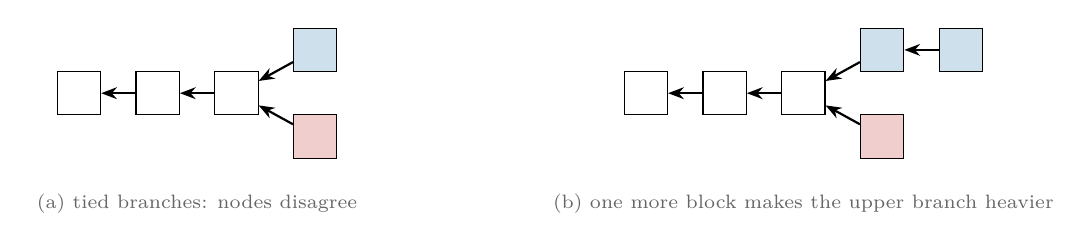
\begin{tikzpicture}[
  blk/.style={draw, rectangle, minimum width=5.5mm, minimum height=5.5mm,
    inner sep=0pt, fill=white},
  hon/.style={blk, fill=tierin!25},
  att/.style={blk, fill=tierspend!25},
  lnk/.style={-{Stealth[length=2mm]}, thick},
  lbl/.style={font=\scriptsize, text=black!60},
]
% panel (a): a tie
\begin{scope}
\node[blk] (g) at (0,0) {};
\node[blk] (b1) at (1,0) {};
\node[blk] (b2) at (2,0) {};
\node[hon] (c1) at (3,0.55) {};
\node[att] (d1) at (3,-0.55) {};
\draw[lnk] (b1) -- (g);
\draw[lnk] (b2) -- (b1);
\draw[lnk] (c1) -- (b2);
\draw[lnk] (d1) -- (b2);
\node[lbl, anchor=north] at (1.5,-1.15) {(a) tied branches: nodes
  disagree};
\end{scope}
% panel (b): resolution
\begin{scope}[xshift=7.2cm]
\node[blk] (g) at (0,0) {};
\node[blk] (b1) at (1,0) {};
\node[blk] (b2) at (2,0) {};
\node[hon] (c1) at (3,0.55) {};
\node[hon] (c2) at (4,0.55) {};
\node[att] (d1) at (3,-0.55) {};
\draw[lnk] (b1) -- (g);
\draw[lnk] (b2) -- (b1);
\draw[lnk] (c1) -- (b2);
\draw[lnk] (c2) -- (c1);
\draw[lnk] (d1) -- (b2);
\node[lbl, anchor=north] at (2,-1.15) {(b) one more block makes the
  upper branch heavier};
\end{scope}
\end{tikzpicture}
\caption{Branch selection. Arrows point from child to parent. In
panel~(a) two blocks extend the same parent and the branches carry equal
work; each node keeps the one it saw first. In panel~(b) a new block
lands on the upper branch, which now has strictly more cumulative work;
during propagation, every node that knows this state selects the upper
branch, unless the lower branch has meanwhile been extended. At constant
difficulty ``more work'' and ``longer'' coincide, which is how the
paper, and this volume's figures, may draw block counts.}
\label{fig:cons-tree}
\end{figure}

\subsection{The attack}\label{sec:cons-attack}

The double-spend attack, as the paper lays it out (\S3):

\begin{enumerate}[itemsep=1pt]
\item broadcast a transaction paying the merchant;
\item secretly mine a branch from the last pre-transaction block,
  containing instead a conflicting transaction paying the attacker
  himself;
\item wait until the merchant's transaction has $n$ confirmations and
  the merchant, satisfied, hands over the goods;
\item in the paper's first-seen tie model, keep extending the secret branch
  until it carries more work than the public one, then broadcast it. Every
  node that sees it switches to it, the
  payment to the merchant is no longer part of history, and the
  attacker has both the goods and the coins.
\end{enumerate}

Nothing in step~4 violates any validity rule --- the released branch is
a perfectly well-formed chain, merely a different one. The only
question is probabilistic: with what probability does the secret branch
ever get ahead? Answering it exactly in that first-seen model is the business of
Sections~\ref{sec:cons-race} and~\ref{sec:cons-confirm}; the toolkit
comes first.

\section{A probability toolkit}\label{sec:cons-toolkit}

The analysis ahead needs four tools: memoryless clocks (to model block
discovery), a reduction from continuous time to a coin sequence, the
negative binomial distribution (to count the attacker's progress), and
one normalisation lemma about races. Their foundations are the
\emph{Math Guide}'s: probability spaces, conditioning, independence,
random variables, and expectation are constructed there from the
definition of probability onward (\S``Probability, asymptotics, and
computation''), and the extension beyond finite spaces --- countable
additivity, continuity along monotone events, density-defined laws, and
infinite sequences of independent trials --- is its
\S``Beyond finite spaces: countable additivity, limits, and densities''.
What no lower volume owns are the four instruments themselves; each is
constructed here on that base, only as far as the critical path
requires.

\subsection{Memoryless clocks and the attribution
sequence}\label{sec:cons-clocks}

\begin{definition}[Exponential clock]\label{def:cons-exp}
A random variable $X$ is \emph{exponential with rate} $\lambda > 0$ if
$\Pr[X > t] = e^{-\lambda t}$ for all $t \geq 0$ --- a law defined by
the density $\lambda e^{-\lambda t}$ on $t \geq 0$ in the sense of the
\emph{Math Guide}'s density definition, with mean $1/\lambda$.
\end{definition}

\begin{lemma}[Memorylessness]\label{lem:cons-memoryless}
An exponential $X$ satisfies
$\Pr[X > s + t \mid X > s] = \Pr[X > t]$ for all $s, t \geq 0$: having
waited without success teaches nothing about the remaining wait.
\end{lemma}

\begin{proof}
$\Pr[X > s+t \mid X > s]
 = e^{-\lambda(s+t)} / e^{-\lambda s} = e^{-\lambda t}$.
\end{proof}

\begin{lemma}[Race of two clocks]\label{lem:cons-race}
Let $X$ and $Y$ be independent exponentials with rates $\lambda$ and
$\mu$. Then
\[
  \Pr[X < Y] \;=\; \frac{\lambda}{\lambda + \mu},
\]
and the winning time $\min(X, Y)$ is exponential with rate
$\lambda + \mu$.
\end{lemma}

\begin{proof}
Integrating over the time at which $X$ fires,
\[
  \Pr[X < Y]
  = \int_0^\infty \lambda e^{-\lambda t}\, \Pr[Y > t] \,dt
  = \int_0^\infty \lambda e^{-(\lambda+\mu)t} \,dt
  = \frac{\lambda}{\lambda + \mu}.
\]
For the minimum,
$\Pr[\min(X,Y) > t] = \Pr[X > t]\Pr[Y > t] = e^{-(\lambda+\mu)t}$.
Moreover, the joint density that $X$ wins at time $t$ factors as
\[
  \lambda e^{-(\lambda+\mu)t}
  = \frac{\lambda}{\lambda+\mu}\,
    (\lambda+\mu)e^{-(\lambda+\mu)t},
\]
and similarly for $Y$. Thus the winner is independent of the winning time.
\end{proof}

\begin{proposition}[The attribution sequence]\label{prop:cons-attrib}
Model the honest network and attacker as independent exponential clocks
with rates $p/T_0$ and $q/T_0$, restarting when either fires
(Section~\ref{sec:cons-race}). Successive block attributions form an
infinite sequence of independent, identically distributed Bernoulli trials
in the \emph{Math Guide}'s sense: attacker with probability $q$, honest
network with probability $p$, independent of all earlier attributions
and all elapsed times.
\end{proposition}

\begin{proof}
By Lemma~\ref{lem:cons-race} the first block is the attacker's with
probability $(q/T_0)/(p/T_0 + q/T_0) = q$. When a block is found, the
finder's clock restarts by construction, and the loser's remaining wait
is distributed as a fresh clock by Lemma~\ref{lem:cons-memoryless}; the
state after each block is therefore probabilistically identical to the
start, independent of the past. The density factorisation in
Lemma~\ref{lem:cons-race} also makes each winner independent of that race's
elapsed time. The claim follows by induction.
\end{proof}

Proposition~\ref{prop:cons-attrib} is the paper's bridge (its \S3,
with footnote~1 supplying the clock rates) from physical time to
combinatorics: since the question
``does the attacker ever get ahead?''\ concerns only the \emph{order}
of block discoveries, not their times, every result below is a
statement about a $p$/$q$ coin sequence, and the time constant $T_0$
disappears from the answers. Where the exponential model itself comes
from --- and how well Zcash's Equihash fits it --- is a deployment
question, taken up in Section~\ref{sec:cons-equihash}.

\subsection{The negative binomial law}\label{sec:cons-negbin}

\begin{proposition}[Progress of the loser]\label{prop:cons-negbin}
In an attribution sequence with attacker probability $q = 1 - p$, let
$m$ be the number of attacker blocks found strictly before the honest
network's $n$-th block. Then
\[
  P(m) \;=\; \binom{m + n - 1}{m}\, p^n q^m,
  \qquad m = 0, 1, 2, \ldots
\]
--- the \emph{negative binomial} distribution.
\end{proposition}

\begin{proof}
The event fixes the first $m + n$ trials exactly this far: the
$(m+n)$-th trial is honest (the $n$-th honest success), and among the
first $m + n - 1$ trials exactly $m$ are the attacker's, in any of
$\binom{m+n-1}{m}$ orders. Each such order has probability
$p^{n-1} q^m \cdot p$.
\end{proof}

\begin{lemma}[First-to-$n$ race]\label{lem:cons-racenorm}
In the same sequence, let $H_n$ be the event that the honest network
reaches $n$ blocks before the attacker does, and $A_n$ the reverse.
Then $H_n$ and $A_n$ partition the sample space, and
\[
  \Pr[H_n] = \sum_{m=0}^{n-1} \binom{m+n-1}{m} p^n q^m,
  \qquad
  \Pr[A_n] = \sum_{h=0}^{n-1} \binom{h+n-1}{h} q^n p^h,
  \qquad
  \Pr[H_n] + \Pr[A_n] = 1.
\]
\end{lemma}

\begin{proof}
Among the first $2n - 1$ trials one side already has $n$ successes, so
the race terminates; a tie is impossible because block counts advance
one at a time. The event $H_n$ says the $n$-th honest block arrives
while the attacker holds $m \leq n - 1$; summing
Proposition~\ref{prop:cons-negbin} over those $m$ gives the first sum,
and $A_n$ is the same computation with the roles of $p$ and $q$
swapped.
\end{proof}

\begin{remark}[From hash trials to exponential clocks]%
\label{rem:cons-hashtrials}
The exponential model is itself a limit, not an axiom. A miner's work is
modelled as a stream of candidate evaluations, each an independent Bernoulli
trial with a tiny success probability; the number of trials to the
first success is geometric, and a geometric law with small success
probability, viewed at the scale of its mean, converges to the
exponential of Definition~\ref{def:cons-exp}. The step that matters is
\emph{progress-freeness}: a candidate that fails must carry no
information usable by the next one. Whether Zcash's Equihash satisfies
this is examined with the deployed parameters in
Section~\ref{sec:cons-equihash}.
\end{remark}

\section{Playing catch-up}\label{sec:cons-race}

The attacker of Section~\ref{sec:cons-attack} finds himself, at the
moment the merchant ships, some number of blocks behind the public
chain, and wins if his branch ever overtakes it. This section computes
the probability of that event as a function of the deficit; the next
section supplies the distribution of the deficit itself.

Both computations run under the paper's two standing assumptions,
stated here nearly verbatim (the environment form is ours,
Remark~\ref{rem:cons-paper}):

\begin{assumption}[Constant hashrates]\label{ass:cons-hashrate}
The total hashrate of the honest network and the attacker is constant.
Combined they have a hashrate of $H$, of which $pH$ belongs to the
honest network and $qH$ to the attacker, where $0 < p,q < 1$ and
$p + q = 1$.
\end{assumption}

\begin{assumption}[Constant difficulty]\label{ass:cons-difficulty}
The mining difficulty is constant, and such that with hashrate $H$ the
average time to find a block is $T_0$.
\end{assumption}

Under Assumption~\ref{ass:cons-difficulty} every block carries equal
work, so ``most work'' and ``longest'' coincide and the race can be
scored in block counts. Section~\ref{sec:cons-difficulty} explains how
the deployed chain departs from these assumptions --- difficulty adjusts
after every block and hashrate drifts --- and why the formulas should be
read as an equal-difficulty baseline rather than an exact deployment model.

\begin{definition}[The deficit walk]\label{def:cons-walk}
Let $z$ denote the honest chain's lead in blocks over the attacker's
branch. By Proposition~\ref{prop:cons-attrib}, each newly found block
moves $z$ up by $1$ with probability $p$ (honest block) or down by $1$
with probability $q$ (attacker block), independently of the past:
\[
  z_{i+1} \;=\;
  \begin{cases}
    z_i + 1 & \text{with probability } p,\\
    z_i - 1 & \text{with probability } q.
  \end{cases}
\]
The attack succeeds the moment $z$ reaches $-1$: the secret branch is
then strictly ahead, and releasing it rewrites history.
\end{definition}

\begin{theorem}[Catch-up probability; Rosenfeld \S3]\label{thm:cons-catchup}
Let $a_z$ be the probability that the walk of
Definition~\ref{def:cons-walk}, started at deficit $z$, ever reaches
$-1$. Then
\begin{equation}\label{eq:cons-az}
  a_z \;=\; \min(q/p,\, 1)^{\max(z+1,\,0)} \;=\;
  \begin{cases}
    1 & \text{if } z < 0 \text{ or } q \geq p,\\
    (q/p)^{z+1} & \text{if } z \geq 0 \text{ and } q < p.
  \end{cases}
\end{equation}
\end{theorem}

\begin{proof}
For $z < 0$ the walk has already succeeded, so $a_z = 1$; assume
$z \geq 0$. Fix an integer $N > z$ and absorb the walk at both $-1$ and
$N$; let $h_N(z)$ be the probability of reaching $-1$ before $N$.
Conditioning on the first step,
\[
  h_N(z) = p\, h_N(z+1) + q\, h_N(z-1)
  \qquad (0 \leq z \leq N - 1),
  \qquad h_N(-1) = 1, \quad h_N(N) = 0,
\]
a second-order linear recurrence. The trial solution $h_N(z) = t^z$
satisfies it exactly when $t$ is a root of the \emph{characteristic
polynomial} $p t^2 - t + q = p(t - 1)(t - q/p)$.

If $q \neq p$ the roots $1$ and $q/p$ are distinct, so
$h_N(z) = A + B (q/p)^z$; the boundary conditions give
\[
  h_N(z) \;=\;
  \frac{(q/p)^z - (q/p)^N}{(q/p)^{-1} - (q/p)^N}.
\]
If $q = p$ the root is double and $h_N(z) = A + Bz$, giving
$h_N(z) = (N - z)/(N + 1)$.

Now let $N \to \infty$. The events $E_N = \{\text{reach } -1 \text{
before } N\}$ are nondecreasing in $N$, and their union is the event
that the walk ever reaches $-1$: a walk that does so does it at a
finite time, having visited finitely many states, so $E_N$ holds for
every $N$ above the largest state visited. By continuity along
monotone events (\emph{Math Guide}, \S``Beyond finite spaces: countable
additivity, limits, and densities''),
$a_z = \lim_{N\to\infty} h_N(z)$. For $q < p$ the term
$(q/p)^N$ vanishes and the quotient tends to $(q/p)^{z+1}$; for
$q = p$, $(N-z)/(N+1) \to 1$; for $q > p$, dividing numerator and
denominator by $(q/p)^N$ sends both to $-1$, so the quotient tends to
$1$.
\end{proof}

\begin{corollary}[Half or more always catches up]\label{cor:cons-majority}
When $q \geq p$, the attacker overtakes the public chain with
probability $1$ from any finite deficit. No confirmation count defends
when the attacker controls at least half of the hashrate.
\end{corollary}

\begin{corollary}[Geometric decay in the deficit]\label{cor:cons-decay}
When $q < p$, each additional block of deficit multiplies the catch-up
probability by $q/p$. Concretely (script-computed): at $q = 10\%$,
$a_0 = 1/9 \approx 0.1111$ and $a_5 \approx 1.88 \times 10^{-6}$; at
$q = 30\%$, $a_0 = 3/7 \approx 0.4286$ and
$a_5 \approx 6.20 \times 10^{-3}$.
\end{corollary}

\begin{corollary}[Blocks, not time]\label{cor:cons-timefree}
Equation~\eqref{eq:cons-az} contains neither $T_0$ nor any other time
scale: the security of a deficit is a function of block \emph{counts}
alone. Two chains with different block spacings but the same $q$ offer
identical security per confirmation --- and therefore different
security per minute (Section~\ref{sec:cons-zcashtime}).
\end{corollary}

\begin{figure}[ht]
\centering
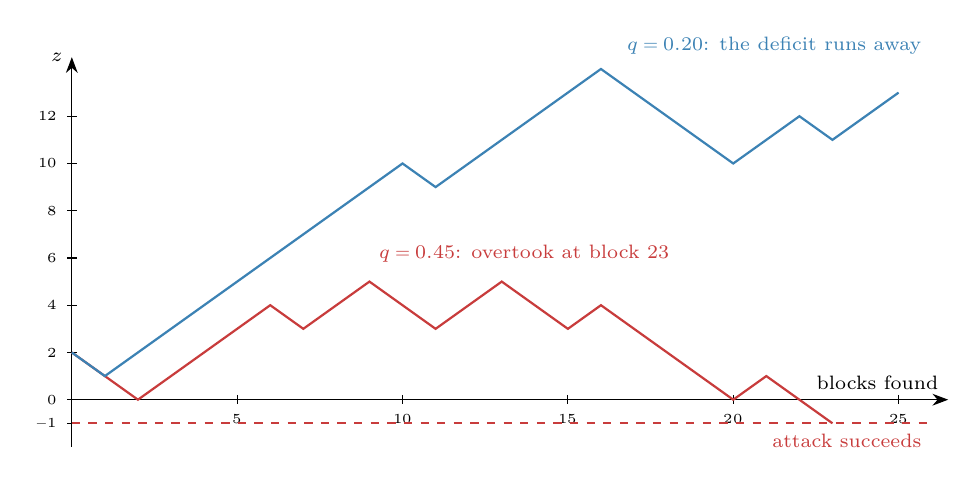
\begin{tikzpicture}[x=0.42cm, y=0.30cm]
% axes
\draw[-{Stealth[length=2mm]}] (0,-2) -- (0,14.5)
  node[left, font=\scriptsize] {$z$};
\draw[-{Stealth[length=2mm]}] (0,0) -- (26.5,0)
  node[above left, font=\scriptsize] {blocks found};
\foreach \y in {-1, 0, 2, 4, 6, 8, 10, 12}
  \draw (0.15,\y) -- (-0.15,\y)
    node[left, font=\tiny] {$\y$};
\foreach \x in {5, 10, 15, 20, 25}
  \draw (\x,0.2) -- (\x,-0.2) node[below, font=\tiny] {$\x$};
% success threshold
\draw[dashed, thick, tierspend]
  (0,-1) -- (26,-1) node[below left, font=\scriptsize, text=tierspend]
  {attack succeeds};
% success walk, q=0.45 seed 0
\draw[thick, tierspend]
  plot coordinates {(0,2) (1,1) (2,0) (3,1) (4,2) (5,3) (6,4) (7,3)
  (8,4) (9,5) (10,4) (11,3) (12,4) (13,5) (14,4) (15,3) (16,4) (17,3)
  (18,2) (19,1) (20,0) (21,1) (22,0) (23,-1)};
\node[font=\scriptsize, text=tierspend, anchor=south west] at (9,5.4)
  {$q = 0.45$: overtook at block $23$};
% failure walk, q=0.20 seed 0
\draw[thick, tierin]
  plot coordinates {(0,2) (1,1) (2,2) (3,3) (4,4) (5,5) (6,6) (7,7)
  (8,8) (9,9) (10,10) (11,9) (12,10) (13,11) (14,12) (15,13) (16,14)
  (17,13) (18,12) (19,11) (20,10) (21,11) (22,12) (23,11) (24,12)
  (25,13)};
\node[font=\scriptsize, text=tierin, anchor=south west] at (16.5,14.2)
  {$q = 0.20$: the deficit runs away};
\end{tikzpicture}
\caption{Two runs of the deficit walk from $z = 2$, simulated by script
with fixed seeds. At $q = 0.45$ the drift is weak and this run reaches
$-1$ after $23$ blocks --- the attack succeeds; at $q = 0.20$ the
deficit grows roughly linearly, and by Theorem~\ref{thm:cons-catchup}
the chance of ever returning from deficit $13$ is
$(1/4)^{14} \approx 3.7 \times 10^{-9}$.}
\label{fig:cons-walk}
\end{figure}

\FloatBarrier

\section{Waiting for confirmations}\label{sec:cons-confirm}

The merchant's defence is patience: ship only after the paying
transaction has $n$ confirmations (Definition~\ref{def:cons-conf}).
This section computes exactly how much that patience buys in the paper's
first-seen model. The paper's
model of the attack timeline has one convention worth surfacing before
the theorem.

\begin{remark}[The pre-mined block]\label{rem:cons-premine}
The paper assumes the attacker banks one block before the race is
scored: ``we assume one block was pre-mined by the attacker before
commencing the attack'' (\S4). The attacker forks from the public leaf
at the moment the merchant's transaction is broadcast, and a patient
attacker times the broadcast to coincide with a private block he has
just found but not announced. At the moment the honest chain reaches
$n$ confirmations, the attacker who has found $m$ further blocks
therefore holds $m + 1$, and the deficit walk of
Definition~\ref{def:cons-walk} starts at
\[
  z \;=\; n - m - 1.
\]
The convention is a modelling choice, not a law: an attacker with no
banked block starts at $z = n - m$, and every probability below
shrinks accordingly. It is also, as
Theorem~\ref{thm:cons-r} shows, precisely the choice that makes the
final formula collapse into a symmetric race.
\end{remark}

By Proposition~\ref{prop:cons-negbin}, the number $m$ of attacker
blocks found while the honest network finds its $n$ is negative
binomial. Averaging the catch-up probability of
Theorem~\ref{thm:cons-catchup} over $m$ gives the central result for the
specification and Rosenfeld first-seen tie rule. Section~\ref{sec:cons-selection}
explains the additional success opportunity supplied by Zebra's tie-break.
The model is not an exact deployed rollback probability.

\begin{theorem}[Double-spend success probability; Rosenfeld
eq.~(1)]\label{thm:cons-r}
Let the merchant wait for $n \geq 1$ confirmations, under
Assumptions \ref{ass:cons-hashrate} and~\ref{ass:cons-difficulty} and
the convention of Remark~\ref{rem:cons-premine}, with a private branch
accepted only after it becomes strictly heavier. The probability that
the attacker's branch eventually overtakes the public chain is
$r(q, n) = 1$ if $q \geq p$, and otherwise
\begin{equation}\label{eq:cons-r}
  r(q, n)
  \;=\; 1 - \sum_{m=0}^{n-1} \binom{m+n-1}{m}
        \left( p^n q^m - p^m q^n \right)
  \;=\; 2 \sum_{m=0}^{n-1} \binom{m+n-1}{m} p^m q^n .
\end{equation}
\end{theorem}

\begin{proof}
Conditioning on $m$ and applying Theorem~\ref{thm:cons-catchup} at
$z = n - m - 1$,
\[
  r \;=\; \sum_{m=0}^{\infty} P(m)\, a_{n-m-1}
  \;=\; \underbrace{\sum_{m=0}^{n-1} P(m) \left( \frac{q}{p}
        \right)^{\!n-m}}_{\text{behind: must catch up}}
  \;+\; \underbrace{\sum_{m=n}^{\infty} P(m)}_{\text{already ahead}},
\]
valid for $q < p$; when $q \geq p$ every $a_{n-m-1} = 1$ and $r =
\sum_m P(m) = 1$ immediately. For the first sum, each term transforms
exactly:
\[
  \binom{m+n-1}{m} p^n q^m \left( \frac{q}{p} \right)^{\!n-m}
  \;=\; \binom{m+n-1}{m} p^m q^n ,
\]
which by Lemma~\ref{lem:cons-racenorm} is the probability that the
attacker's $n$-th block arrives while the honest network holds $m$;
summed over $m \leq n - 1$, the first sum is $\Pr[A_n]$, the
probability that the attacker wins the first-to-$n$ race. The
second sum is $\Pr[m \geq n] = 1 - \Pr[H_n] = \Pr[A_n]$ by the same
lemma. Hence $r = 2 \Pr[A_n]$, the right-hand form
of~\eqref{eq:cons-r}; the middle form follows from
$\Pr[A_n] = 1 - \Pr[H_n]$ applied to one of the two copies. The
printed upper limit in the paper's equation~(1) is $n$ rather than
$n - 1$; the $m = n$ term is identically zero, so the forms agree.
\end{proof}

\begin{remark}[The race doubling]\label{rem:cons-doubling}
The proof exposes a structure the paper's algebra passes through
silently: under the one-pre-mined-block convention, the
\emph{catch-up half} --- the honest chain reaches $n$ first and the attacker
later overtakes --- has exactly the same probability as the
\emph{already-ahead half}, in which the attacker reaches $n$ first. A
first-to-$n$ winner may have fallen behind and recovered along the way; neither
half asserts otherwise. Thus the double-spend probability is twice the chance
of winning a first-to-$n$ race. The
identity also absorbs the boundary case: at $q = p$ each race half is
exactly $\tfrac12$, giving $r = 1$ with no case split, continuously
with the $q > p$ regime. The algebra here is the paper's; reading its
two sums as the two halves of one race, and the observation that the
pre-mine convention is what makes them equal, are this volume's
presentational additions (verified by script over random $(q, n)$; the
two sums agree to floating-point precision).
\end{remark}

\begin{example}[A full race, exactly]\label{ex:cons-worked}
Take $q = 1/5$ (a twenty-percent attacker) and $n = 6$. The deficit
starts at $z = 5 - m$, the catch-up factor is
$(q/p)^{6-m} = 4^{-(6-m)}$, and every quantity below is an exact
rational, printed to six decimals (script-computed):
\begin{center}
\small
\begin{tabular}{@{}rrrr@{}}
\toprule
$m$ & $P(m)$ & $a_{5-m} = 4^{-(6-m)}$ & product \\
\midrule
$0$ & $0.262144$ & $0.000244$ & $0.000064$ \\
$1$ & $0.314573$ & $0.000977$ & $0.000307$ \\
$2$ & $0.220201$ & $0.003906$ & $0.000860$ \\
$3$ & $0.117441$ & $0.015625$ & $0.001835$ \\
$4$ & $0.052848$ & $0.062500$ & $0.003303$ \\
$5$ & $0.021139$ & $0.250000$ & $0.005285$ \\
\midrule
\multicolumn{3}{@{}l}{catch-up half (sum of products)} & $0.011654$ \\
\multicolumn{3}{@{}l}{already-ahead half, $\Pr[m \geq 6]$} & $0.011654$ \\
\midrule
\multicolumn{3}{@{}l}{$r(0.2,\, 6)$} & $0.023308$ \\
\bottomrule
\end{tabular}
\end{center}
The two halves agree to every printed digit --- they are equal exactly,
by Remark~\ref{rem:cons-doubling} --- and the closed
form~\eqref{eq:cons-r} evaluates to the same $0.023308$. A merchant
facing a possible twenty-percent adversary who ships after six
confirmations is assigned a $2.33\%$ strict-overtake probability by this
model.
\end{example}

\begin{remark}[Satoshi's approximation]\label{rem:cons-satoshi}
The whitepaper's \S11 computes the same quantity with one
approximation and two offsetting conventions: the attacker's progress
is approximated as Poisson with mean $\lambda = n q / p$ (the law
$\Pr[k] = e^{-\lambda} \lambda^k / k!$ on the nonnegative integers);
no block is pre-mined, but success is scored at \emph{breakeven}
rather than
strictly ahead, and those two conventions cancel exactly --- the
whitepaper's catch-up factor for $m$ attacker blocks is
$(q/p)^{n-m}$, term for term the factor of
Remark~\ref{rem:cons-premine}. The Poisson approximation is the
entire gap. In each of the following script-computed comparisons it pushes
the estimate down: at $q = 10\%$, $n = 6$, the whitepaper's formula gives
$0.0243\%$ against the exact $0.0591\%$ --- an understatement by a
factor of about $2.4$; at $q = 30\%$, $n = 6$: $13.211\%$ against
$15.645\%$; at $q = 10\%$, $n = 10$: $0.0001\%$ against $0.0008\%$.
The direction is not uniform over all $(q,n)$; the reason to prefer the
negative binomial model is that it is exact under the stated assumptions, not
that the approximation is always one-sided.
\end{remark}

\begin{table}[ht]
\centering
\footnotesize
\setlength{\tabcolsep}{4.4pt}
\begin{tabular}{@{}r rrrrrrrrrr@{}}
\toprule
$q$ & $n{=}1$ & $2$ & $3$ & $4$ & $5$ & $6$ & $7$ & $8$ & $9$ & $10$ \\
\midrule
$2\%$ & $4.000$ & $0.237$ & $0.016$ & $0.0011$ &
  $8\!\cdot\!10^{-5}$ & \multicolumn{5}{c}{$< 10^{-5}$} \\
$5\%$ & $10.000$ & $1.450$ & $0.232$ & $0.039$ & $0.0066$ &
  $0.0012$ & $2.1\!\cdot\!10^{-4}$ & $4\!\cdot\!10^{-5}$ &
  \multicolumn{2}{c@{}}{$< 10^{-5}$} \\
$10\%$ & $20.000$ & $5.600$ & $1.712$ & $0.546$ & $0.178$ & $0.059$ &
  $0.020$ & $0.0067$ & $0.0023$ & $0.0008$ \\
$20\%$ & $40.000$ & $20.800$ & $11.584$ & $6.669$ & $3.916$ & $2.331$ &
  $1.401$ & $0.848$ & $0.516$ & $0.316$ \\
$30\%$ & $60.000$ & $43.200$ & $32.616$ & $25.207$ & $19.762$ &
  $15.645$ & $12.475$ & $10.003$ & $8.055$ & $6.511$ \\
$40\%$ & $80.000$ & $70.400$ & $63.488$ & $57.958$ & $53.314$ &
  $49.300$ & $45.769$ & $42.621$ & $39.787$ & $37.218$ \\
$45\%$ & $90.000$ & $85.050$ & $81.375$ & $78.342$ & $75.716$ &
  $73.375$ & $71.252$ & $69.299$ & $67.487$ & $65.793$ \\
$48\%$ & $96.000$ & $94.003$ & $92.508$ & $91.264$ & $90.177$ &
  $89.201$ & $88.307$ & $87.478$ & $86.703$ & $85.972$ \\
$50\%$ & \multicolumn{10}{c@{}}{$100$ for every $n$} \\
\bottomrule
\end{tabular}
\caption{The double-spend success probability $r(q, n)$, in percent,
computed by script from Theorem~\ref{thm:cons-r}. On the rows the
paper's Table~1 also prints ($q \in \{2, 10, 20, 30, 40, 48, 50\}\%$),
the script reproduces its values cell-for-cell; the $5\%$ and $45\%$
rows are this volume's additions.}
\label{tab:cons-r}
\end{table}

\begin{figure}[ht]
\centering
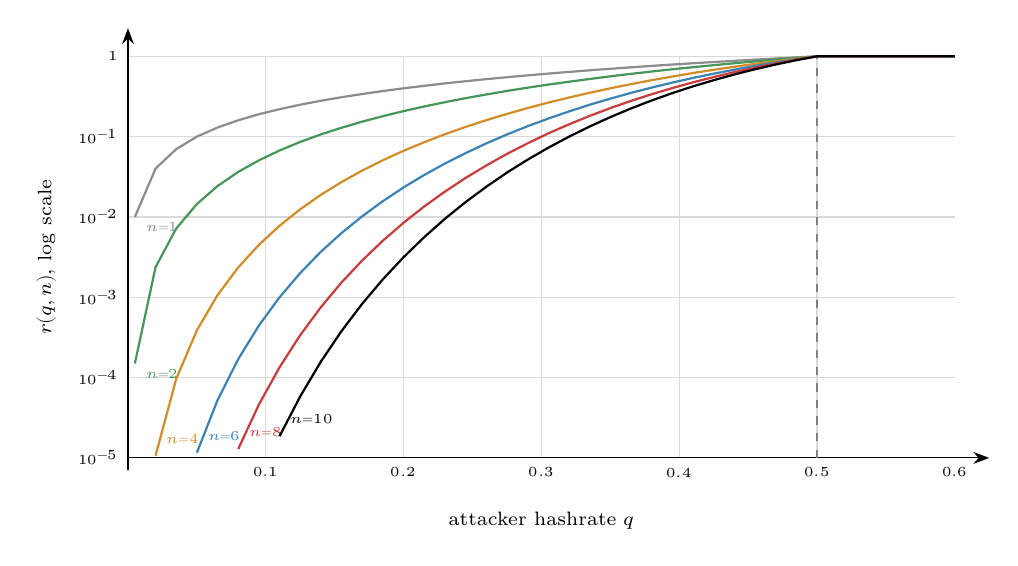
\begin{tikzpicture}[x=17.5cm, y=1.02cm]
% frame and grid
\draw[black!15] (0,-5) grid[xstep=0.1, ystep=1] (0.6,0);
\draw[-{Stealth[length=2mm]}] (0,-5.15) -- (0,0.35);
\draw[-{Stealth[length=2mm]}] (0,-5) -- (0.625,-5);
\foreach \y/\l in {0/{1}, -1/{10^{-1}}, -2/{10^{-2}}, -3/{10^{-3}},
  -4/{10^{-4}}, -5/{10^{-5}}}
  \node[left, font=\tiny] at (0,\y) {$\l$};
\foreach \x in {0.1, 0.2, 0.3, 0.4, 0.5, 0.6}
  \node[below, font=\tiny] at (\x,-5) {$\x$};
\node[below, font=\scriptsize] at (0.3,-5.55) {attacker hashrate $q$};
\node[left, font=\scriptsize, rotate=90, anchor=south] at (-0.045,-2.5)
  {$r(q,n)$, log scale};
\draw[dashed, black!50] (0.5,-5) -- (0.5,0);
% n = 1
\draw[thick, black!45] plot coordinates {(0.005,-2.000) (0.020,-1.398)
(0.035,-1.155) (0.050,-1.000) (0.065,-0.886) (0.080,-0.796)
(0.095,-0.721) (0.110,-0.658) (0.125,-0.602) (0.140,-0.553)
(0.155,-0.509) (0.170,-0.469) (0.185,-0.432) (0.200,-0.398)
(0.215,-0.367) (0.230,-0.337) (0.245,-0.310) (0.260,-0.284)
(0.275,-0.260) (0.290,-0.237) (0.305,-0.215) (0.320,-0.194)
(0.335,-0.174) (0.350,-0.155) (0.365,-0.137) (0.380,-0.119)
(0.395,-0.102) (0.410,-0.086) (0.425,-0.071) (0.440,-0.056)
(0.455,-0.041) (0.470,-0.027) (0.485,-0.013) (0.500,0.000)
(0.600,0.000)};
\node[font=\tiny, text=black!45, anchor=west] at (0.006,-2.12)
  {$n{=}1$};
% n = 2
\draw[thick, tierrecv] plot coordinates {(0.005,-3.825) (0.020,-2.626)
(0.035,-2.144) (0.050,-1.839) (0.065,-1.615) (0.080,-1.439)
(0.095,-1.295) (0.110,-1.172) (0.125,-1.066) (0.140,-0.972)
(0.155,-0.889) (0.170,-0.813) (0.185,-0.745) (0.200,-0.682)
(0.215,-0.624) (0.230,-0.571) (0.245,-0.521) (0.260,-0.475)
(0.275,-0.431) (0.290,-0.390) (0.305,-0.352) (0.320,-0.316)
(0.335,-0.282) (0.350,-0.249) (0.365,-0.218) (0.380,-0.189)
(0.395,-0.161) (0.410,-0.135) (0.425,-0.110) (0.440,-0.086)
(0.455,-0.063) (0.470,-0.041) (0.485,-0.020) (0.500,0.000)
(0.600,0.000)};
\node[font=\tiny, text=tierrecv, anchor=west] at (0.006,-3.95)
  {$n{=}2$};
% n = 4
\draw[thick, tierfull] plot coordinates {(0.020,-4.972) (0.035,-4.016)
(0.050,-3.412) (0.065,-2.973) (0.080,-2.628) (0.095,-2.347)
(0.110,-2.109) (0.125,-1.904) (0.140,-1.724) (0.155,-1.565)
(0.170,-1.422) (0.185,-1.293) (0.200,-1.176) (0.215,-1.069)
(0.230,-0.970) (0.245,-0.879) (0.260,-0.795) (0.275,-0.717)
(0.290,-0.644) (0.305,-0.576) (0.320,-0.513) (0.335,-0.454)
(0.350,-0.398) (0.365,-0.346) (0.380,-0.297) (0.395,-0.252)
(0.410,-0.208) (0.425,-0.168) (0.440,-0.130) (0.455,-0.094)
(0.470,-0.061) (0.485,-0.029) (0.500,0.000) (0.600,0.000)};
\node[font=\tiny, text=tierfull, anchor=south west] at (0.021,-4.95)
  {$n{=}4$};
% n = 6
\draw[thick, tierin] plot coordinates {(0.050,-4.935) (0.065,-4.281)
(0.080,-3.770) (0.095,-3.352) (0.110,-3.000) (0.125,-2.698)
(0.140,-2.433) (0.155,-2.200) (0.170,-1.991) (0.185,-1.803)
(0.200,-1.632) (0.215,-1.477) (0.230,-1.335) (0.245,-1.205)
(0.260,-1.084) (0.275,-0.973) (0.290,-0.870) (0.305,-0.775)
(0.320,-0.686) (0.335,-0.603) (0.350,-0.527) (0.365,-0.455)
(0.380,-0.389) (0.395,-0.327) (0.410,-0.269) (0.425,-0.216)
(0.440,-0.166) (0.455,-0.119) (0.470,-0.076) (0.485,-0.037)
(0.500,0.000) (0.600,0.000)};
\node[font=\tiny, text=tierin, anchor=south west] at (0.051,-4.91)
  {$n{=}6$};
% n = 8
\draw[thick, tierspend] plot coordinates {(0.080,-4.889)
(0.095,-4.336) (0.110,-3.871) (0.125,-3.471) (0.140,-3.123)
(0.155,-2.815) (0.170,-2.541) (0.185,-2.295) (0.200,-2.072)
(0.215,-1.869) (0.230,-1.684) (0.245,-1.514) (0.260,-1.359)
(0.275,-1.215) (0.290,-1.083) (0.305,-0.960) (0.320,-0.847)
(0.335,-0.742) (0.350,-0.645) (0.365,-0.555) (0.380,-0.472)
(0.395,-0.395) (0.410,-0.324) (0.425,-0.258) (0.440,-0.197)
(0.455,-0.141) (0.470,-0.090) (0.485,-0.043) (0.500,0.000)
(0.600,0.000)};
\node[font=\tiny, text=tierspend, anchor=south west] at (0.081,-4.86)
  {$n{=}8$};
% n = 10
\draw[thick, black] plot coordinates {(0.110,-4.730) (0.125,-4.234)
(0.140,-3.801) (0.155,-3.420) (0.170,-3.080) (0.185,-2.776)
(0.200,-2.501) (0.215,-2.251) (0.230,-2.023) (0.245,-1.815)
(0.260,-1.624) (0.275,-1.448) (0.290,-1.287) (0.305,-1.138)
(0.320,-1.001) (0.335,-0.874) (0.350,-0.757) (0.365,-0.649)
(0.380,-0.550) (0.395,-0.458) (0.410,-0.374) (0.425,-0.297)
(0.440,-0.226) (0.455,-0.161) (0.470,-0.102) (0.485,-0.048)
(0.500,0.000) (0.600,0.000)};
\node[font=\tiny, anchor=south west] at (0.111,-4.70) {$n{=}10$};
\end{tikzpicture}
\caption{The success probability $r(q, n)$ against the attacker's
hashrate share $q$, for $n \in \{1, 2, 4, 6, 8, 10\}$ confirmations,
logarithmic vertical scale clipped at $10^{-5}$; coordinates computed
by script from Theorem~\ref{thm:cons-r}. Every curve reaches $1$ at
$q = \tfrac12$ (dashed) and stays there: beyond the majority line,
confirmations are worthless. Below it, each added confirmation drops
$r$ by a roughly constant factor --- the curves are near-equally
spaced in log scale --- and the factor improves as $q$ falls.}
\label{fig:cons-rq}
\end{figure}

\FloatBarrier

\section{What the numbers say}\label{sec:cons-analysis}

Theorem~\ref{thm:cons-r} compresses the security of Nakamoto consensus
into one two-parameter function, and its qualitative lessons are all
visible in Table~\ref{tab:cons-r} and Figure~\ref{fig:cons-rq}. This
section states them precisely, then instantiates the one lesson that is
specific to Zcash.

\begin{table}[ht]
\centering
\small
\begin{tabular}{@{}r rrr@{}}
\toprule
$q$ & $r < 10\%$ & $r < 1\%$ & $r < 0.1\%$ \\
\midrule
$2\%$ & $1$ & $2$ & $3$ \\
$5\%$ & $2$ & $3$ & $4$ \\
$8\%$ & $2$ & $3$ & $5$ \\
$10\%$ & $2$ & $4$ & $6$ \\
$15\%$ & $3$ & $6$ & $9$ \\
$20\%$ & $4$ & $8$ & $13$ \\
$25\%$ & $5$ & $12$ & $20$ \\
$30\%$ & $9$ & $20$ & $32$ \\
$35\%$ & $15$ & $36$ & $58$ \\
$40\%$ & $34$ & $82$ & $133$ \\
$45\%$ & $135$ & $331$ & $539$ \\
\bottomrule
\end{tabular}
\caption{The least number of confirmations pushing $r(q, n)$ below
three targets, computed by script. The growth is logarithmic in the
inverse target risk but explosive in $q$: a $10\%$ attacker is answered by $6$
confirmations, a $45\%$ attacker by $539$, and at $50\%$ by no number at all.}
\label{tab:cons-nreq}
\end{table}

\begin{proposition}[No finite count is final]\label{prop:cons-nozero}
For every $0 < q < p$ and every $n$,
$r(q, n) \geq 2 q^n > 0$.
\end{proposition}

\begin{proof}
By Theorem~\ref{thm:cons-r}, $r = 2 \Pr[A_n]$, and one way for the
attacker to win the first-to-$n$ race is to find the first $n$ blocks
outright, an event of probability $q^n$.
\end{proof}

\begin{proposition}[Divergence at the majority line]%
\label{prop:cons-divergence}
Fix a target $0 < \varepsilon < 1$. For $0 < q < \tfrac12$, let
$n_\varepsilon(q)$ be the least $n$ with $r(q, n) < \varepsilon$. Then
$n_\varepsilon(q) \to \infty$ as $q \uparrow \tfrac12$.
\end{proposition}

\begin{proof}
First, $n_\varepsilon(q)$ exists. The event $A_n$ that the attacker reaches
$n$ blocks first is the event that at least $n$ of the first $2n-1$ block
discoveries are the attacker's. Since $q<p$, each such length-$(2n-1)$
sequence has probability at most $q^n p^{n-1}$, and there are fewer than
$2^{2n-1}$ sequences. Hence
\[
  r(q,n)=2\Pr[A_n] \leq \frac{(4pq)^n}{p} \longrightarrow 0,
\]
because $4pq<1$.

For fixed $n$ the function $q \mapsto r(q, n)$ is a polynomial on
$[0, \tfrac12]$, hence continuous, and $r(\tfrac12, n) = 1$: at
$q = p$ each half of the race of Remark~\ref{rem:cons-doubling} has
probability exactly $\tfrac12$ by Lemma~\ref{lem:cons-racenorm} and
symmetry. Given any $N$, for each $1\leq n\leq N$ there is a
$\delta_n > 0$ with $r(q, n) > \varepsilon$ whenever
$q > \tfrac12 - \delta_n$. Taking
$\delta=\min_{1\leq n\leq N}\delta_n>0$ excludes every
$n\leq N$ throughout that neighbourhood, so
$n_\varepsilon(q)>N$. Since $N$ was arbitrary, the claimed divergence
follows.
\end{proof}

\begin{remark}[Nothing is special about six]\label{rem:cons-six}
The paper (\S5): ``There is nothing special about the default,
often-cited figure of 6 confirmations. It was chosen based on the
assumption that an attacker is unlikely to amass more than 10\% of the
hashrate, and that a negligible risk of less than 0.1\% is acceptable.
Both these figures are arbitrary''\ --- six confirmations are
``overkill for casual attackers, and at the same time powerless against
more dedicated attackers''. Table~\ref{tab:cons-nreq} is the honest
replacement: pick the adversary you defend against and the risk you
accept, and read off $n$; the pair $(q, \varepsilon)$ is a policy, not
a law of nature.
\end{remark}

\subsection{Zcash time: 25-second blocks}\label{sec:cons-zcashtime}

Corollary~\ref{cor:cons-timefree} says security is purchased in blocks.
The wall-clock price is set by the target spacing: $25$ seconds in
\href{https://zips.z.cash/zip-0218}{ZIP-218}. Since public discoveries
arrive at rate $p/T_0$, waiting for $n$ confirmations takes $nT_0/p$
seconds in expectation in this model. Three confirmations cost a nominal
$75$ seconds and ten cost $250$ seconds when all hashpower publishes on the
public chain. With a $10\%$ withholding attacker, the expected wait is
instead divided by $0.9$.

For example, a nominal thirty-minute wait buys $72$ confirmations at
$25$-second spacing, compared with three at Bitcoin's $600$-second spacing.
The corresponding strict-overtake probabilities against a $10\%$ attacker
are approximately $9.35\times10^{-34}$ and $1.712\%$, respectively; either
count takes $30/0.9\approx33.3$ minutes in expectation under withholding.
These are model calculations, not guarantees about either network.

The comparison holds $q$ fixed. It contains no network and therefore does
not price honest blocks racing one another during propagation. Quantifying
that lost work requires a propagation distribution and mining topology.
Moreover, a policy waiting for a fixed amount of accumulated miner reward
asks a different question: decreasing the reward per block in proportion
to the target spacing requires proportionally more blocks to reach that
amount. Ignoring transaction fees (value paid for transaction inclusion)
and rounding, the shorter spacing then cancels out
of the mean wait. The monetary and fixed-hashrate models are not
interchangeable.

\begin{remark}[Where the model bends]\label{rem:cons-modellimits}
Three assumptions do not survive contact with the deployed chain; they
determine how cautiously the calculations may be transferred to it.
(i)~\emph{Difficulty is not constant}: Zcash retunes the target after
every block (Section~\ref{sec:cons-difficulty}). The race is scored in
work, not block counts, and $q$ may be interpreted approximately as the
attacker's share of work production while the branches' block weights
remain close; once their difficulty schedules diverge, the equal-step
random-walk formula is no longer exact.
(ii)~\emph{Hashrate is not constant}: $q$ in the theorems is whatever
share the attacker sustains for the attack's duration; the paper's own
caveat is that $T_0$ re-enters only if the attacker cannot sustain his
hashrate long enough, which it judges unlikely for a serious attacker.
(iii)~\emph{Propagation is not instantaneous}: honest self-orphaning
wastes honest work and thereby raises the attacker's effective share;
its size is not quantified here. A fourth gap is not the model's: the
attacker of this volume follows the
protocol's validity rules perfectly and attacks only the
\emph{choice} between valid histories. Attacks on the rules themselves
are other volumes' subjects.
\end{remark}

\section{The economics of the attack}\label{sec:cons-econ}

The probabilities of Section~\ref{sec:cons-confirm} answer the
adversarial merchant, who assumes the customer is an attacker. The
paper's \S6 answers the realistic one: when is the attack worth
mounting at all? Throughout this section $q < p$ --- ``[o]therwise,
all bets are off'' (\S6) --- and the model is deliberately stylised;
its own caveats close the section.

The attacker targets $k$ merchants simultaneously with payments of $v$
each, all invalidated by the same secret branch; the goods are worth
$\alpha v$ to him, $0 < \alpha \leq 1$; he gives up after mining $o$
blocks in vain; and each of his blocks would earn the block income $B$
if it ended up in the accepted chain. If the attack succeeds his
blocks are all accepted (he keeps goods \emph{and} coins \emph{and}
rewards); if it fails he has paid $kv$, keeps goods worth
$k \alpha v$, and his $o$ orphaned blocks forfeit $oB$.
For an exact finite-stop profit calculation, $r$ would have to be the
success probability of that stopping policy. Following the paper, the
tables below instead insert the unlimited-horizon $r(q,n)$ as a heuristic
proxy. They are not an exact evaluation of a strategy that always stops
after $o=20$ private blocks.

\begin{proposition}[Profitability; Rosenfeld \S6]\label{prop:cons-profit}
Given success probability $r$ and these stipulated payoffs, the
attacker's expected profit over not attacking is
\[
  k \alpha v - (1 - r)(k v + o B)
  \;=\; k v (\alpha + r - 1) - (1 - r)\, o B ,
\]
positive if and only if
\[
  v \;>\; \frac{(1 - r)\, o B}{k (\alpha + r - 1)}
\]
(when $\alpha + r > 1$; when $\alpha + r \leq 1$ the modeled attack is
never strictly profitable). This modeled attack is not strictly profitable
whenever
\begin{equation}\label{eq:cons-vmax}
  v \;\leq\; \frac{o (1 - r) B}{k (\alpha + r - 1)}
  \;\overset{\alpha = 1}{=}\;
  \frac{o}{k} \cdot \frac{B (1 - r)}{r},
\end{equation}
which with the paper's choices $o = 20$, $k = 5$, $\alpha = 1$,
$B = 25$~BTC is its equation~(2), $v \leq 100 (1/r - 1)$~BTC.
\end{proposition}

\begin{proof}
The gain $k \alpha v$ is certain (the goods are obtained either way);
the loss $k v + o B$ is paid exactly when the attack fails, with
probability $1 - r$. Rearranging the positivity condition gives the
threshold; substituting the paper's constants gives
$20 \cdot 25 \cdot (1-r) / (5r) = 100(1-r)/r$.
\end{proof}

\subsection{Reward-normalised exposure}\label{sec:cons-econzec}

The \emph{block subsidy} is value issued by the protocol in a block,
distinct from fees transferred by its transactions. Its \emph{scheduled}
component is base issuance determined by height, before any reserve payout.
A \emph{funding
stream} is a required allocation of a share of that subsidy to a designated
recipient. The \emph{coinbase} is the block's first transaction, which
distributes the available subsidy and fees according to the applicable
rules. The \emph{reserve} is the accounting balance of funds removed from
circulation and awaiting reissuance.

The income $B$ forfeited by an orphaned block is the amount its miner would
have retained: miner subsidy plus retained transaction fees, not the
subsidy allocated to other recipients. Under NU7 this depends on scheduled
issuance, the prior reserve balance, and the applicable fee-removal rule
(Section~\ref{sec:cons-nu7-nsm}). A universal ZEC figure would therefore
hide assumptions about both chain state and unresolved draft rules.

Instead, Table~\ref{tab:cons-vmax} measures transaction value in units of
the chosen block income $B$. With the paper's $o=20$, $k=5$, and
$\alpha=1$, equation~\eqref{eq:cons-vmax} becomes
\[
  \frac{v}{B}\leq4\,\frac{1-r}{r}.
\]
Once a particular threat model supplies $B$, multiplying by it gives the
corresponding monetary threshold. Treating $B$ as constant over the attack
remains a modelling assumption.

\begin{table}[ht]
\centering
\small
\begin{tabular}{@{}r rrrrrr@{}}
\toprule
$q$ & $n{=}1$ & $2$ & $4$ & $6$ & $8$ & $10$ \\
\midrule
$5\%$ & $36$ & $271$ & $10{,}327$ & $344{,}743$ &
  $10{,}931{,}506$ & $336{,}737{,}801$ \\
$10\%$ & $16$ & $67$ & $729$ & $6{,}759$ & $59{,}475$ & $508{,}917$ \\
$20\%$ & $6$ & $15$ & $55$ & $167$ & $467$ & $1{,}262$ \\
$30\%$ & $2$ & $5$ & $11$ & $21$ & $35$ & $57$ \\
$40\%$ & $1$ & $1$ & $2$ & $4$ & $5$ & $6$ \\
\bottomrule
\end{tabular}
\caption{The largest whole-number multiple of block income $B$ with
non-positive heuristic expected profit:
$\lfloor4(1-r)/r\rfloor$, computed by script. The table is dimensionless:
it neither fixes a ZEC subsidy nor predicts future fee income. Values
inherit every assumption of the model; the caveats of
Remark~\ref{rem:cons-econcaveats} apply in full.}
\label{tab:cons-vmax}
\end{table}

Within the model, a handful of confirmations makes the attack unprofitable
against small attackers at any plausible payment size; against a $30\%$
attacker, six confirmations make modeled expected profit non-positive only
up to about $21$ times the assumed block income $B$. The required count grows only logarithmically in the
value at stake, by the geometric decay of Theorem~\ref{thm:cons-r}. These are
neither exact finite-stop profit calculations nor bounds on deployed
rollback risk; the deployed tie-break, changing difficulty, and rollback
rails require separate modelling.

\begin{remark}[Majority is a different problem]\label{rem:cons-majority}
At $q=p$, eventual strict overtake has probability $1$, but the walk has zero
drift; that fact alone does not give the attacker a lasting monopoly. When
$q>p$, the economics change character entirely: the paper notes a strict
majority attacker can double-spend at no cost beyond normal
mining, reject every other miner's blocks to take the whole issuance,
and exclude transactions at will, driving honest miners out and
entrenching himself --- so a majority attack ``is best seen as an
attempt to destroy'' the currency, motivated from outside it (a short
position, a competing system), not an attempt to profit inside it.
Confirmation policy is not the defence at that point; the defence is
the cost of assembling the majority, which lies outside this model.
\end{remark}

\begin{remark}[The model's own caveats]\label{rem:cons-econcaveats}
The paper flags each stylisation itself. The give-up point $o = 20$
``is a significant simplification'' (an optimal attacker balances
completion against compounding losses); the safe values ``should be
taken with a grain of salt, because of the many modeling
assumptions''; and a model resting on mining \emph{costs} rather than
forfeited \emph{rewards} would make the required confirmations linear,
not logarithmic, in the transaction value --- ``very poor security,
hence in a situation where this is relevant, we have already lost
anyway'' (\S6). The bound's role is the shape it reveals ---
logarithmic patience buys exponential safety --- not its third
significant digit.
\end{remark}

\FloatBarrier

\section{NU7: 25-second blocks and bounded shielded work}
\label{sec:cons-deployed}\label{sec:cons-nu7}

The \href{https://zips.z.cash/zip-0259}{ZIP-259} draft combines three
changes: shorter blocks with limits on shielded work
(\href{https://zips.z.cash/zip-0218}{ZIP-218}), reissuance that preserves the
halving schedule --- periodic divisions of scheduled subsidy by two
(\href{https://github.com/zcash/zips/pull/1354}{ZIP-237}) ---
and rejection of version~4 transactions
(\href{https://zips.z.cash/zip-2003}{ZIP-2003}). This section describes that
proposal, not a deployed upgrade. Its activation height, denoted $A$, is
unassigned on each network at the source boundary in
Section~\ref{sec:cons-sources}.

NU7 introduces no new transaction format: versions~5 and~6 remain available.
Their signatures nevertheless commit to a \emph{consensus branch identifier},
a value identifying the network upgrade's rules. An unchanged encoding
therefore does not make a pre-NU7 signature valid under NU7.
Disabling version~4 also disables spending funds in Sprout, an older
shielded pool, because the newer formats cannot represent its transfers;
it does not transfer their value to a reserve or remove it from the supply.

\subsection{Chain selection and the tie-break}\label{sec:cons-selection}

The most-work rule remains Definition~\ref{def:cons-best}: compare the
sum of the blocks' work, not their count. Changing target spacing changes
neither the work definition nor this ordering.

\begin{remark}[The implementation tie-break]\label{rem:cons-tiebreak}
The specification and Rosenfeld's model prefer the first-seen block at
equal cumulative work. The examined Zebra implementation instead uses the
larger tip hash. This distinction concerns local chain choice, not the
validity of a block.
The divergence matters to the attack model. At equal work, an attacker can
compare its private tip hash with the public tip and reveal immediately when
its hash wins the deployed deterministic tie-break; the strict-overtake
boundary $z=-1$ used above does not count that success opportunity. Therefore
$r(q,n)$ is exact for the stated strict-overtake model and is a lower
bound if only its tie-break is replaced by Zebra's, keeping equal
difficulty, unlimited rollback, and the other assumptions fixed.
It is not thereby a lower bound on the full deployed process: changing
difficulty and rollback limits also change the success event. Quantifying the
extra probability, including any scope to choose among candidate private tips,
requires a different stopping rule and is outside this volume.
\end{remark}

\subsection{Difficulty in motion}\label{sec:cons-difficulty}
\label{sec:cons-nu7-time}

Assumption~\ref{ass:cons-difficulty} freezes difficulty; Zcash retargets
after every block. In \href{https://zips.z.cash/zip-0218}{ZIP-218}, the NU7
target spacing is $25$ seconds and the target-averaging window is $102$
blocks. The timestamps determining the adjustment still come from the
branch being evaluated, including on an attacker's private branch.

Write $N=102$ for the target-averaging window and $T=N\cdot25=2{,}550$
seconds for its nominal timespan.

The specification's
\href{https://zips.z.cash/protocol/protocol.pdf\#diffadjustment}{\S7.7.3}
defines the rest of the calculation. For a block height $h$, let
$m(h)$ be the median timestamp of the eleven preceding blocks: their
sixth-smallest timestamp. Let $\overline{t}(h)$ be the mean target of
the $N$ blocks preceding $h$: the sum of their targets divided by $N$.
Define the observed and damped timespans by
\begin{align*}
 a(h)&=m(h)-m(h-N),\\
 d(h)&=T+\operatorname{trunc}\!\left(\frac{a(h)-T}4\right),
\end{align*}
where $\operatorname{trunc}$ discards the fractional part towards zero.
The bounded timespan $c(h)$ is $d(h)$ clamped between
$\lfloor0.84T\rfloor$ and $\lfloor1.32T\rfloor$: values below the
lower endpoint are replaced by that endpoint, and similarly above the
upper endpoint. The maximum target $\mathsf{PoWLimit}$ is $2^{243}-1$ on
Mainnet, the production network, and $2^{251}-1$ on Testnet, the test network
(\href{https://zips.z.cash/protocol/protocol.pdf\#constants}{\S5.3}).
The target calculation is
\[
  t(h)=\min\!\left(\mathsf{PoWLimit},\;
       \left\lfloor\frac{\overline{t}(h)}{T}\right\rfloor c(h)\right),
\]
followed by the compact encoding defined in the specification's
\href{https://zips.z.cash/protocol/protocol.pdf\#nbits}{\S7.7.4}.
The order of the floor and multiplication matters. At NU7 the clamp
endpoints are $2{,}142$ and $3{,}366$ seconds; the eleven-timestamp median,
fourfold damping, and target cap are unchanged.

Activation does not reset the accumulated work or multiply the target by
three in a single operation. The first NU7 blocks still look back over
pre-NU7 history and adjust through the same bounded rule. Likewise, the
timestamp rules do not shrink with the target spacing: a timestamp must
exceed the median of the preceding eleven and be at most $90$ minutes
above it (\href{https://zips.z.cash/protocol/protocol.pdf\#blockheader}{\S7.6}).
A further non-consensus receipt check rejects blocks more than two hours
ahead of the validator's clock. Testnet's exceptional minimum-difficulty rule
continues to use six target spacings: its delay threshold becomes
$6\cdot25=150$ seconds. This exception does not apply to Mainnet.

\begin{remark}[What per-block retargeting changes]
\label{rem:cons-difffidelity}
The averaging window, damping, and clamp constrain the adjustment but do
not prove that two forked branches retain close targets. Work per block
moves inversely with the target; a branch's timestamps can change both
its future block rate and the work carried by each block. Equal expected
work production does not make the probability of an eventual overtake
independent of these jump sizes. Consequently, the probability tables are
an equal-work baseline, not an exact analysis of private branches whose
difficulty schedules diverge.
\end{remark}

\subsection{Equihash and the memoryless model}\label{sec:cons-equihash}

Zcash's proof of work is Equihash with parameters $n = 200$, $k = 9$
(specification \href{https://zips.z.cash/protocol/protocol.pdf\#pow}{\S7.7}, \href{https://zips.z.cash/protocol/protocol.pdf\#equihash}{\S7.7.1}; the algorithm is Biryukov and
Khovratovich's, ePrint~2015/946), but the quantity the race counts is
gated one step later: ``[t]he difficulty filter is unchanged from
Bitcoin, and is calculated using SHA-256d on the whole block header
(including \texttt{solutionSize} and \texttt{solution})'', required to
be at most $\mathsf{ToTarget}(\texttt{nBits})$ (\href{https://zips.z.cash/protocol/protocol.pdf\#difficulty}{\S7.7.2}). Each
candidate Equihash solution therefore faces a fresh SHA-256d lottery.
Treating distinct headers as independent trials is the usual random-function
model for SHA-256d, not a property asserted by the specification; under that
model these are the Bernoulli trials of Remark~\ref{rem:cons-hashtrials}.

The specification nowhere asserts progress-freeness --- the argument
is this volume's, not a citation. What Equihash changes is the
granularity: candidates arrive in batches, one batch per memory-hard
solver run.
Progress within a run is discarded when a competing block arrives. Under
independent identically distributed runs, the number of runs until an accepted
header is geometric; replacing those discrete completion times by an
exponential clock is a further approximation, coarse within one run and good
only when a run is short relative to the target spacing: $25$ seconds in
the NU7 draft. Run duration is
implementation- and hardware-dependent and is not quantified here. A
proof-of-work whose solve time were comparable to the spacing would make block
discovery visibly non-exponential and pull the attribution sequence away from
Proposition~\ref{prop:cons-attrib}.

\subsection{Reorg rails, maturity, and the finality
floor}\label{sec:cons-rails}

Consensus does not impose a maximum reorganisation depth. ZIP-218
recommends a node-local $600$-block rollback window: at the target spacing
this is $600\cdot25=15{,}000$ seconds, or $250$ minutes. Such a limit bounds
the history that a node automatically reverses; it is not a proof that
older blocks cannot be replaced by a higher-work valid chain. Following
a branch outside that retained history requires different local state or
operator intervention. Actual node implementations may choose a different
window.

\begin{remark}[What the rails buy]\label{rem:cons-railsregister}
A finite rollback policy truncates some paths to eventual overtake,
so the unlimited-rollback probability $r(q,n)$ is not the exact failure
probability of a node enforcing that policy. A limit is also not global
agreement: different nodes may stop on different sides of a long split.
The specification's
\href{https://zips.z.cash/protocol/protocol.pdf\#blockchain}{\S3.3}
adds a separate requirement for validators that risk Mainnet funds or
display transaction information: their chain must include the activation
block of the most recent settled network upgrade. That socially anchored
checkpoint is distinct from probabilistic finality.
\end{remark}

A \emph{transparent output} records its value and destination in cleartext.
The consensus maturity rule prevents spending such an output of a coinbase
until the spending block is at least $100$ heights later
(\href{https://zips.z.cash/protocol/protocol.pdf\#txnconsensus}{\S7.1.2}).
ZIP-218 keeps that count, a nominal $100\cdot25=2{,}500$ seconds. Coinbase
outputs placed directly in a shielded pool do not have this transparent
maturity restriction. A $600$-block rollback window can therefore reverse
an already mature coinbase: maturity permits spending, not finality.

\subsection{Wallet confirmation policy}\label{sec:cons-walletpolicy}

A wallet can distinguish \emph{trusted} outputs that its own transaction
handling can recreate after a rollback from an \emph{untrusted} external
payment that may require the sender to pay again. The examined wallet
backend uses three confirmations for the former and ten for the latter,
with zero-confirmation shielding of transparent funds allowed by its
default policy. These choices are not consensus rules.

Table~\ref{tab:cons-r} quantifies their modelled trade-off: three
confirmations assign a $10\%$ attacker risk $1.712\%$, while ten assign the
same attacker about $0.0008\%$ and a $20\%$ attacker about $0.316\%$.
The count remains a $(q,\varepsilon)$ policy, not a guarantee.

The \emph{anchor} is the note-commitment-tree root against which a spend
proves membership (\emph{Crypto Guide}, \S{}Privacy-preserving membership
via zero-knowledge paths). ZIP-218 keeps the recommended anchor depth
at three blocks. Its recommended transaction-expiry delta is $120$
blocks, a nominal $120\cdot25=3{,}000$ seconds, without overriding an
explicitly configured expiry delta. There is no instruction to divide
every confirmation count by three.

\subsection{A block budget for shielded work}\label{sec:cons-nu7-limits}

A byte limit does not directly bound the computational work inside a
block. The $2{,}000{,}000$-byte limit must therefore be considered alongside
the $25$-second target spacing and the costs of shielded validation and
wallet scanning. ZIP-218
adds limits on the shielded components that drive this work.

An Orchard \emph{Action} pairs one spend slot with one output slot; dummy
slots allow either side to carry no real transfer. Ironwood is the newer
shielded pool using the same Action structure
(\href{https://zips.z.cash/zip-0229}{ZIP-229}). The older Sapling shielded
pool counts spends and outputs separately; its cryptographic construction is
not needed for this accounting.

Let $O$ and $I$ count Orchard and Ironwood Actions in a block, and let $S$
count Sapling spends plus outputs. With the Ironwood coverage proposed in
\href{https://github.com/zcash/zips/pull/1361}{PR~1361}, the complete
shielded budget is
\[
 O\leq330,\qquad I\leq330,\qquad S\leq300,
 \qquad O+I+S\leq330.
\]
The final inequality is shared across pools: their separate maxima cannot
all be filled in one block. Sprout transfers cannot occur because NU7
rejects the version~4 format that represents them.

The Ironwood term remains under review rather than already specified by
the merged ZIP-218 draft. For example, $O=100$, $I=200$, $S=30$ exhausts
the shared budget; increasing $I$ to $201$ violates it even though each per-pool
limit still holds. At two Actions per transaction, a block devoted to
one Orchard-protocol pool fits at most $165$ such transactions under this
budget, or a nominal $165/25=6.6$ transactions per second. This is a
capacity calculation under a specified transaction shape, not a measured
throughput guarantee. Transparent components remain subject to the byte
limit rather than this shielded-action budget.

\subsection{Scheduled issuance with shorter blocks}
\label{sec:cons-nu7-subsidy}

A \emph{zatoshi} is the atomic currency unit: $1$~ZEC equals $10^8$
zatoshi. A \emph{halving} divides the scheduled subsidy by two. Retaining its
nominal wall-clock interval while tripling block frequency requires both
three times as many blocks per interval and one third of the subsidy per
block. ZIP-218 therefore changes the full interval from $1{,}680{,}000$
to $L=5{,}040{,}000$ blocks. These earlier intervals are needed to compute
progress at activation, not to supply an alternative rule. The change
preserves expected timing, not exact calendar dates, because actual block
times remain random.

The progress already made towards the next halving must survive activation.
Let $H_B$ be the Blossom activation height: $653{,}600$ on Mainnet and
$584{,}000$ on Testnet. Before Blossom, halvings were separated by
$840{,}000$ blocks; the initial slow-start schedule, which ramps up the
subsidy during the first $20{,}000$ blocks, contributes a shift of
$10{,}000$ blocks. These constants and the maximum subsidy
$M=1{,}250{,}000{,}000$ zatoshi are defined in the specification's
\href{https://zips.z.cash/protocol/protocol.pdf\#constants}{\S5.3} and
\href{https://zips.z.cash/protocol/protocol.pdf\#subsidies}{\S7.8}.
For a height $h\geq A$, the draft's halving count and scheduled subsidy
$s_h$, measured in zatoshi, are
\begin{align}
 k(h)&=\left\lfloor
       \frac{H_B-10{,}000}{840{,}000}
       +\frac{A-H_B}{1{,}680{,}000}
       +\frac{h-A}{5{,}040{,}000}\right\rfloor,
       \label{eq:cons-nu7-halving}\\
 s_h&=\left\lfloor\frac{M}{2\cdot3\cdot2^{k(h)}}\right\rfloor.
       \label{eq:cons-nu7-subsidy}
\end{align}
The factors $2$ and $3$ account separately for Blossom's and NU7's
spacing changes. If activation occurs during the second-halving era,
$k(h)=2$ gives $s_h=52{,}083{,}333$ zatoshi, or $0.52083333$~ZEC, until
the next halving; $k(h)=3$ gives $26{,}041{,}666$ zatoshi.

The old Mainnet third-halving height $H_3=4{,}406{,}400$ is therefore not
the NU7 third-halving height if $A<H_3$. Converting the remaining interval
gives
\[
 H_3^{\mathrm{NU7}}=A+3(H_3-A)=13{,}219{,}200-2A.
\]
No numerical activation height is assigned here. Nor does retiming the
halving function automatically retime a funding stream whose endpoint is
specified as a literal block height. The draft does not provide such a
change, so the funding-stream endpoints and the rescaled halving heights
must be treated separately.

\subsection{The NSM reserve and delayed reissuance}
\label{sec:cons-nu7-nsm}

The \emph{Network Sustainability Mechanism} (NSM) separates temporarily
removed funds from the still-unissued scheduled subsidy. In the
\href{https://github.com/zcash/zips/pull/1354}{merged ZIP-237 draft}, the
\emph{issued supply} $V_h$ is the total value recorded in the chain's
value pools after block $h$. Each pool is a separately tracked balance
for one part of the protocol; tracking a shielded pool's total does not
reveal the values of its individual notes. The \emph{NSM reserve} $R_h$ records
value removed from circulation and not yet reissued. The reserve is public
consensus state, not a spendable pool or an account with a spending key.
In particular, it is not $21$ million ZEC minus the issued supply: that
larger difference also includes future scheduled issuance.

The initial reserve recovers the historical subsidy and fees that miners
left unclaimed before NU6. Since
\href{https://zips.z.cash/zip-0236}{ZIP-236}, a coinbase must account for
its full available value, so that historical shortfall is fixed. The draft
defines the seed $R_{A-1}$ as total scheduled issuance through the last
pre-NU6 block minus issued supply there. The exact integer seeds for
Mainnet and Testnet remain unspecified.

Let $D\geq A$ be the separately assigned height at which reissuance starts,
and let $d_h$ be the non-negative number of zatoshi removed from circulation
in block $h$ by whatever removal mechanisms have been deployed. With
$L=5{,}040{,}000$ blocks per halving interval, the draft selects
\[
 f=\frac{\lfloor6{,}931{,}680{,}000/L\rfloor}{10^{10}}
   =\frac{1375}{10^{10}}.
\]
Its additional subsidy $u_h$, total block subsidy $b_h$, and reserve update
are
\begin{align}
 u_h&=\begin{cases}0,&h<D,\\
       \lceil f R_{h-1}\rceil,&h\geq D,\end{cases}
       \label{eq:cons-nu7-extra}\\
 b_h&=s_h+u_h,\qquad
 R_h=R_{h-1}-u_h+d_h.\label{eq:cons-nu7-reserve}
\end{align}
All amounts are integers in zatoshi. Reissuance uses the previous block's
reserve, so a removal in the current block cannot finance its own
additional subsidy. Before $D$, removals accumulate without payout. After
$D$, a positive reserve pays at least one zatoshi: because $R$ is an
integer and $0<f<1$, one has $1\leq\lceil fR\rceil\leq R$ for $R>0$.
The draft rejects a negative reserve; it does not silently clamp it to zero.

For a small exact example, take $R_{h-1}=100{,}000{,}000$ zatoshi
($1$~ZEC) and $h\geq D$. The additional subsidy is
$\lceil13.75\rceil=14$ zatoshi. Without a new removal the reserve becomes
$99{,}999{,}986$; with a same-block removal of another $1$~ZEC it becomes
$199{,}999{,}986$, but the current payout remains $14$. This example does
not use the unassigned historical seed.

\paragraph{Why this preserves supply and halvings.}
Transfers between ordinary value pools cancel in their total. A block
increases that total by its subsidy and reduces it by its removals:
\[
 V_h-V_{h-1}=s_h+u_h-d_h,
 \qquad (V_h+R_h)-(V_{h-1}+R_{h-1})=s_h.
\]
The second identity follows by adding the reserve update; reissuance moves
value between the two ledgers without creating a second copy. Scheduled
issuance retains its halvings, with the reserve paying an additional
amount on top. Funding streams, wherever active, take their prescribed
fractions of the \emph{total} subsidy $b_h$, not only $s_h$. The resulting
subsidy depends on prior chain state as well as height.

To understand the chosen rate, temporarily ignore integer rounding and
new removals. The recurrence becomes $R_{h+j}=(1-f)^jR_h$, so keeping about
half the reserve after $L$ blocks requires
$f=1-2^{-1/L}\approx(\ln2)/L$. The draft implements an integer-scaled
approximation with numerator $1375$. Indeed,
$(1-1375/10^{10})^{5{,}040{,}000}\approx0.50007$.
This is a half-life of the reserve without new contributions, not a new
halving rule for the scheduled subsidy; small reserves depart from the
smooth curve because every positive payout rounds up.

\paragraph{Unresolved deployment and fee details.}
ZIP-259 selects a reissuance date corresponding to February~2031, but the
network-specific height $D$ remains unassigned.
The drafts do not yet specify a complete, consistent NU7 removal rule:
\href{https://zips.z.cash/zip-0235}{ZIP-235} requires removal of at least
$60\%$ of fees through an explicit coinbase amount, while ZIP-259 describes
a block-level contribution requiring no new transaction data. The reserve
equations therefore leave $d_h$ as a defined input. Neither a particular
fee-removal mechanism nor an exact NU7 miner income is inferred from these
incomplete rules.

\section{Layer boundary}\label{sec:cons-relations}

Every theorem above rests on the \emph{Math Guide}'s probability section:
the definition of probability, its extension beyond finite spaces, and the
continuity theorem used in the catch-up proof. This volume supplies the
best-chain model and the quantitative bounds in
Tables~\ref{tab:cons-r}, \ref{tab:cons-nreq}, and~\ref{tab:cons-vmax}.
Policies that decide which chain view to trust or when to treat a transaction
as final lie above that boundary.

\end{document}
